\begin{figure}[htbp]

\begin{center}
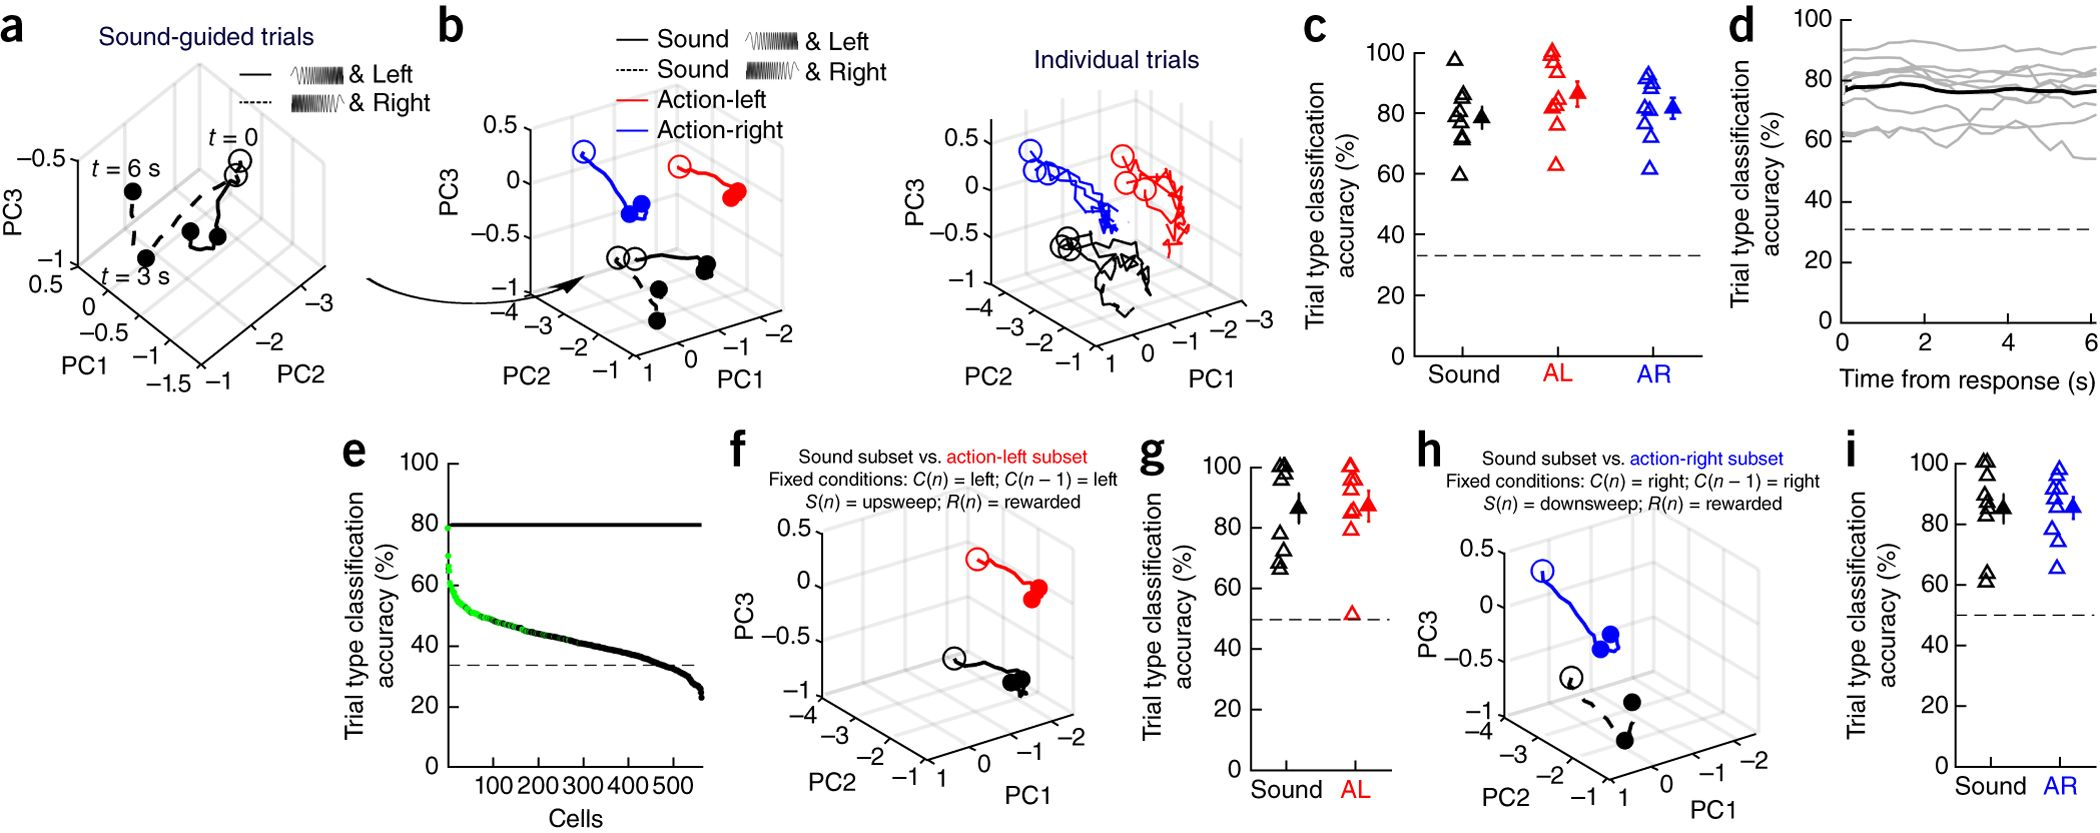
\includegraphics[width=\textwidth]{Figures/Chapter3/NN_fig5} 
\end{center}

\caption[Rule implementations were associated with distinct population activity patterns]
{
Rule implementations were associated with distinct population activity patterns.
(a) Neuronal circuit trajectories for 56 simultaneously imaged cells in one experiment. Trajectories were determined from trial-averaged $\Delta F/F$ for 44 correct left (solid line) and 59 correct right (dotted line) responses in sound-guided trials. Open circles, time of response $t_0$. Filled circles, 3 and 6 s after response. PC, principal component. (b) Same axes as \emph{a}, with additional trajectories from 51 correct action-left (red) and 51 correct action-right (blue) trials. Left, trajectories calculated using trial-averaged $\Delta F/F$. Right, three representative single-trial trajectories from each trial type. (c) Median accuracy of decoding trial type from individual population activity vectors. S, sound; AL, action-left; AR, action-right. Open triangles, individual experiments; filled triangles, $\mathit{mean}\pm\mathit{SEM}$; dotted line, chance-level accuracy. (d) Temporal dependence of ensemble decoding accuracy. Gray, individual experiments. Black, mean. Dotted line, chance-level accuracy. (e) Median accuracy of decoding trial type from fluorescence transients of single neurons. Green circles, trial-type-selective cells; i.e., 95\% percentile confidence intervals are above chance level of 33.3\%. Black circles, other cells. Black line, mean decoding accuracy using ensemble activity. Dotted line, chance-level accuracy. (f--g) Same as \emph{b--c} for trials in which stimulus was upsweep, choice was left, outcome was reward for the current trial and choice was left for the prior trial. Trial type could be decoded well above chance (sound: 87 ± 5\%, action-left: 88 ± 5\%; versus chance level of 50\%, $p = 7 \times 10^{-5}$, $7 \times 10^{-5}$, $t_8 = 7.50$, 7.52, one-sample t-test). (h--i) Same as \emph{b--c} for trials in which stimulus was downsweep, choice was right, outcome was reward for the current trial and choice was right for the prior trial. Trial type could be decoded well above chance (sound: $85 \pm 5\%$, action-right: $86 \pm 4\%$; vs. chance level of 50\%, $p = 7 \times 10^{-5}$, $8 \times 10^{-6}$, $t_8 = 7.54$, 10.01, one-sample t-test). $N = 9$ sessions from 5 mice.
}

\label{fig:NN_fig5}
\end{figure}